\documentclass[utf8]{frontiersHLTH} % for Health articles
\usepackage{url,hyperref,lineno,microtype,longtable,booktabs,bookmark,float}
\usepackage[onehalfspacing]{setspace}

\linenumbers
\def\keyFont{\fontsize{8}{11}\helveticabold }
\def\Address{$address$}
\def\firstAuthorLast{$first_author$ {et~al.}} %use et al only if is more than 1 author
\def\corrAuthor{Christoph Helma, in silico toxicology gmbh, Rastatterstr. 41, CH-4057 Basel, Switzerland}
\def\corrEmail{helma@in-silico.ch}
\extraAuth{}% If there are more than 1 corresponding author, comment this line and uncomment the next one.

% fix frontiersHLTH bugs

% tightlist missing
% http://tex.stackexchange.com/questions/257418/error-tightlist-converting-md-file-into-pdf-using-pandoc
\providecommand{\tightlist}{%
  \setlength{\itemsep}{0pt}\setlength{\parskip}{0pt}}

% description environment missing
\makeatletter
\newenvironment{description}
	{\list{}{\labelwidth\z@ \itemindent-\leftmargin
		\let\makelabel\descriptionlabel}}
	{\endlist}
\newcommand*\descriptionlabel[1]{\hspace\labelsep
	\normalfont\bfseries #1}
\setlength{\labelsep}{.5em}% Also taken from article.cls
\makeatother

\date{$date$}

\begin{document}
\onecolumn
\firstpage{1}

\title[nano-lazar]{$title$}

\author[\firstAuthorLast ]{$authors$} %This field will be automatically populated
\address{} %This field will be automatically populated
\correspondance{} %This field will be automatically populated

\maketitle

\begin{abstract}
$abstract$
\tiny
 \keyFont{ \section{Keywords:} $keywords$} %All article types: you may provide up to 8 keywords; at least 5 are mandatory.
\end{abstract}

$body$


\bibliographystyle{frontiersinHLTH&FPHY} % for Health, Physics and Mathematics articles
\bibliography{$bibliography$}

\newpage

\section{Figures}\label{figures}

\begin{figure}[H]

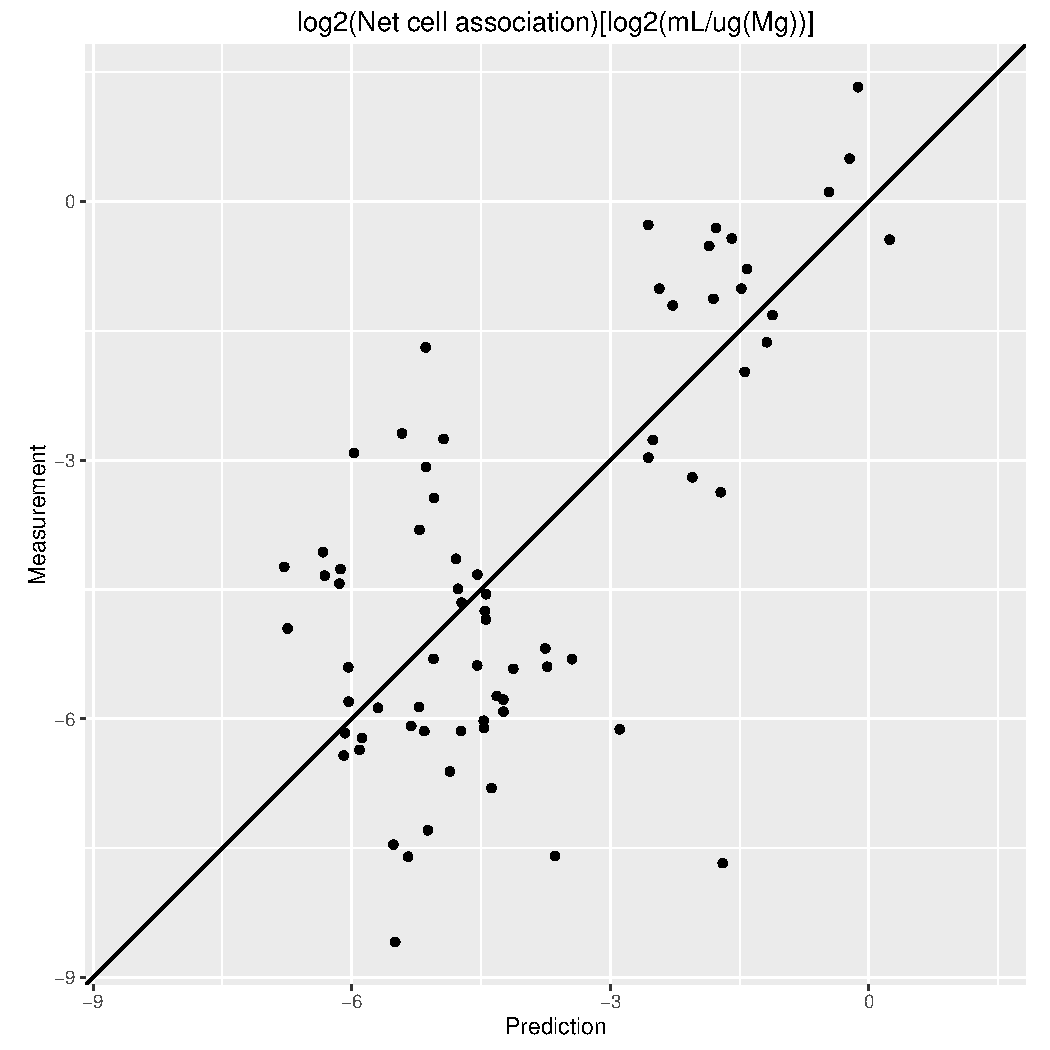
\includegraphics[width=0.3000\textwidth]{figures/MP2D-rf-0.pdf}\label{fig:fingerprint0}
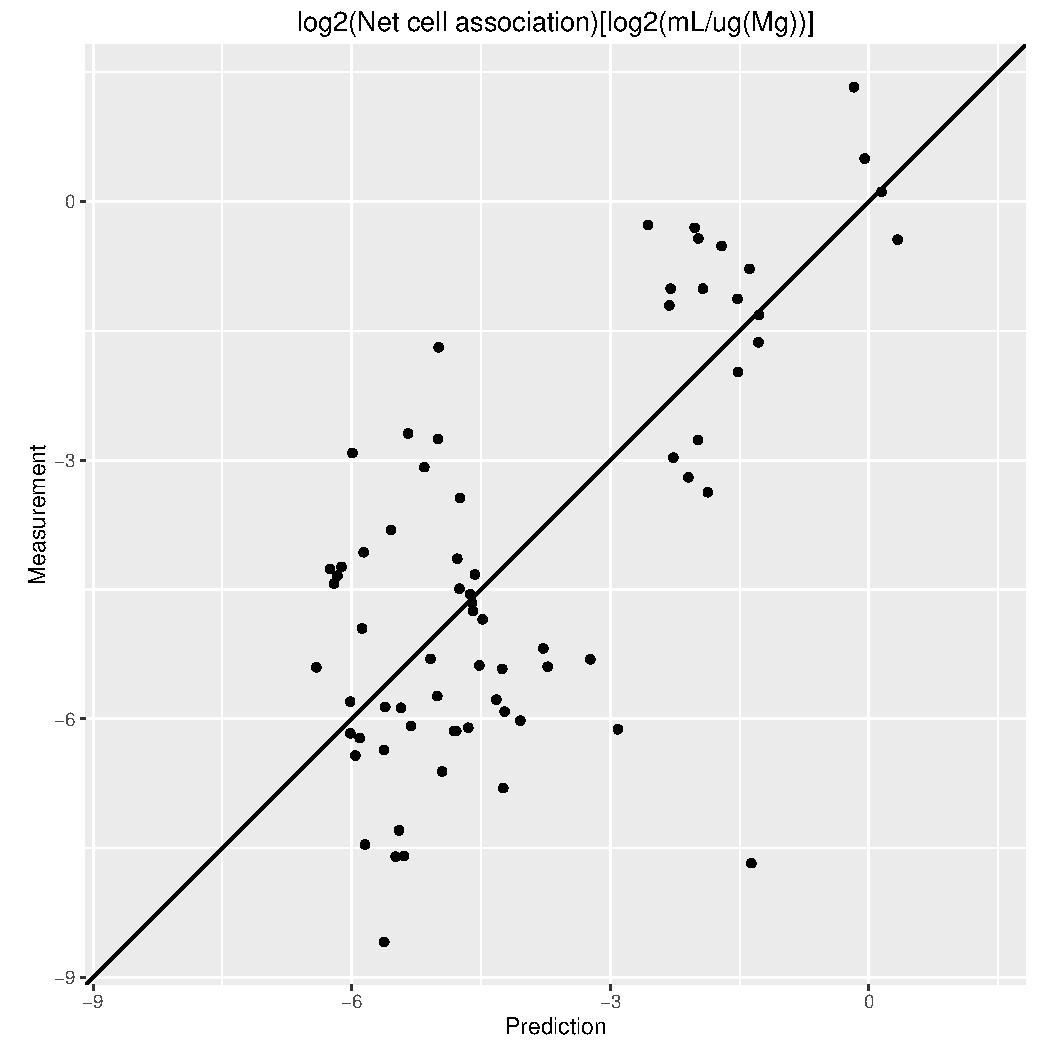
\includegraphics[width=0.3000\textwidth]{figures/MP2D-rf-1.pdf}\label{fig:fingerprint1}
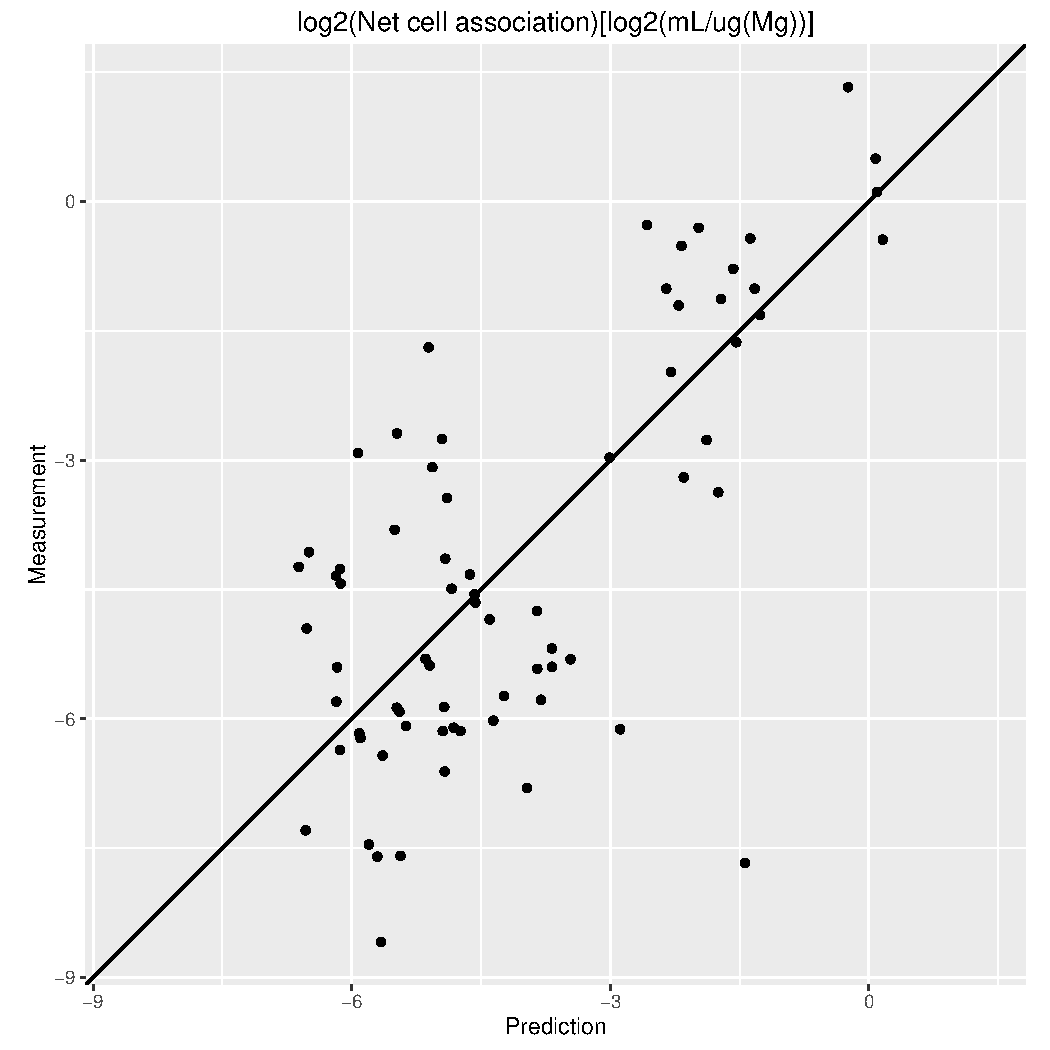
\includegraphics[width=0.3000\textwidth]{figures/MP2D-rf-2.pdf}\label{fig:fingerprint2}
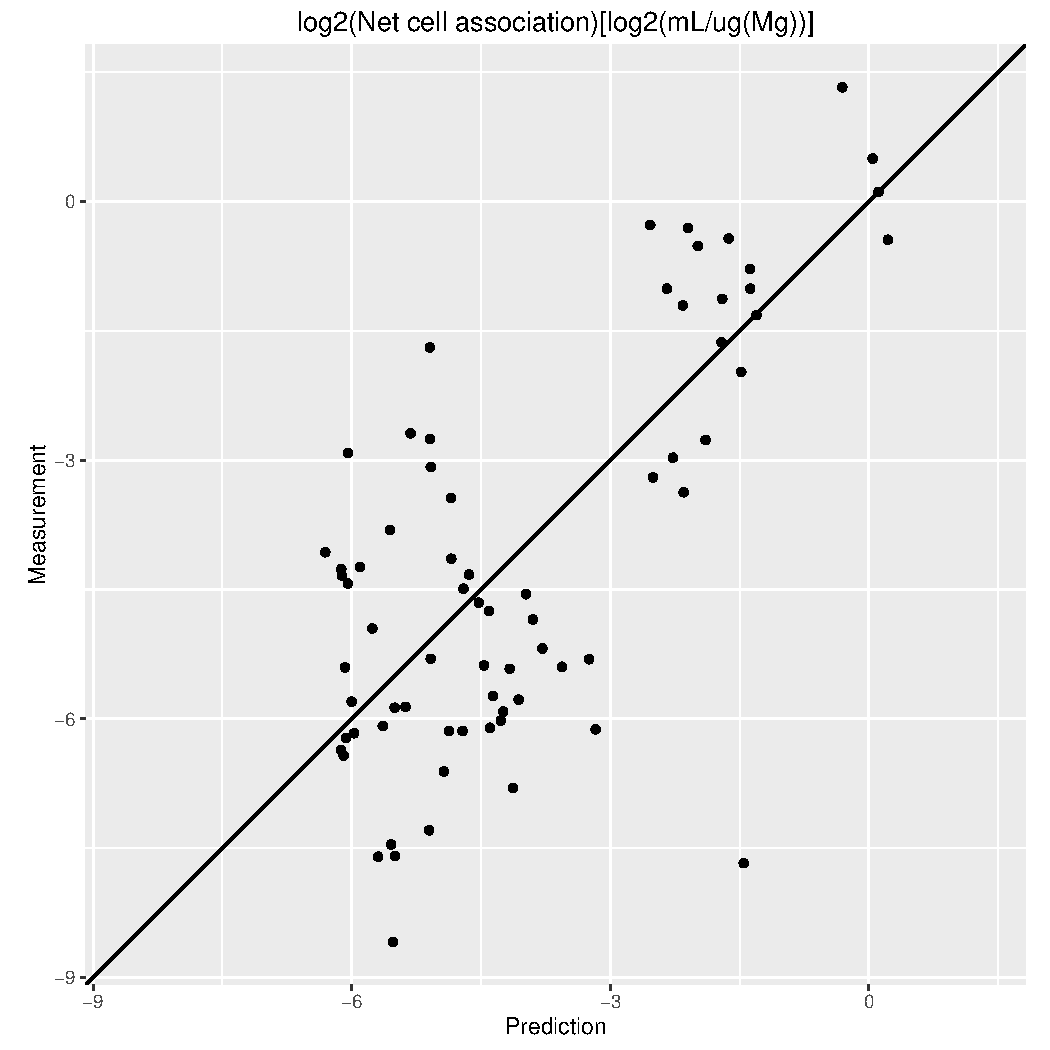
\includegraphics[width=0.3000\textwidth]{figures/MP2D-rf-3.pdf}\label{fig:fingerprint3}
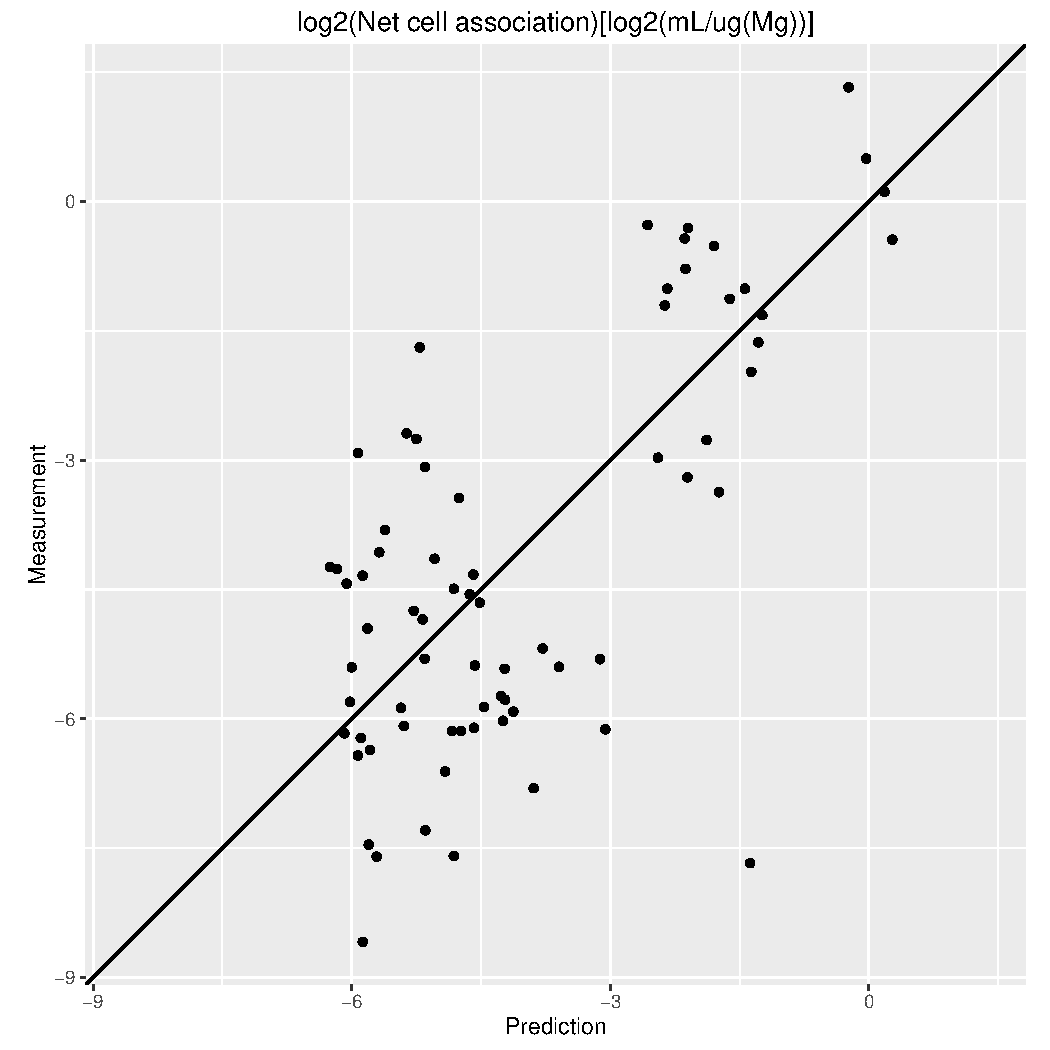
\includegraphics[width=0.3000\textwidth]{figures/MP2D-rf-4.pdf}\label{fig:fingerprint4}

\caption{Correlation of predicted vs.~measured values for five
independent crossvalidations with \emph{MP2D} fingerprint descriptors
and local \emph{random forest} models}

\label{fig:fingerprint}

\end{figure}

\begin{figure}[H]

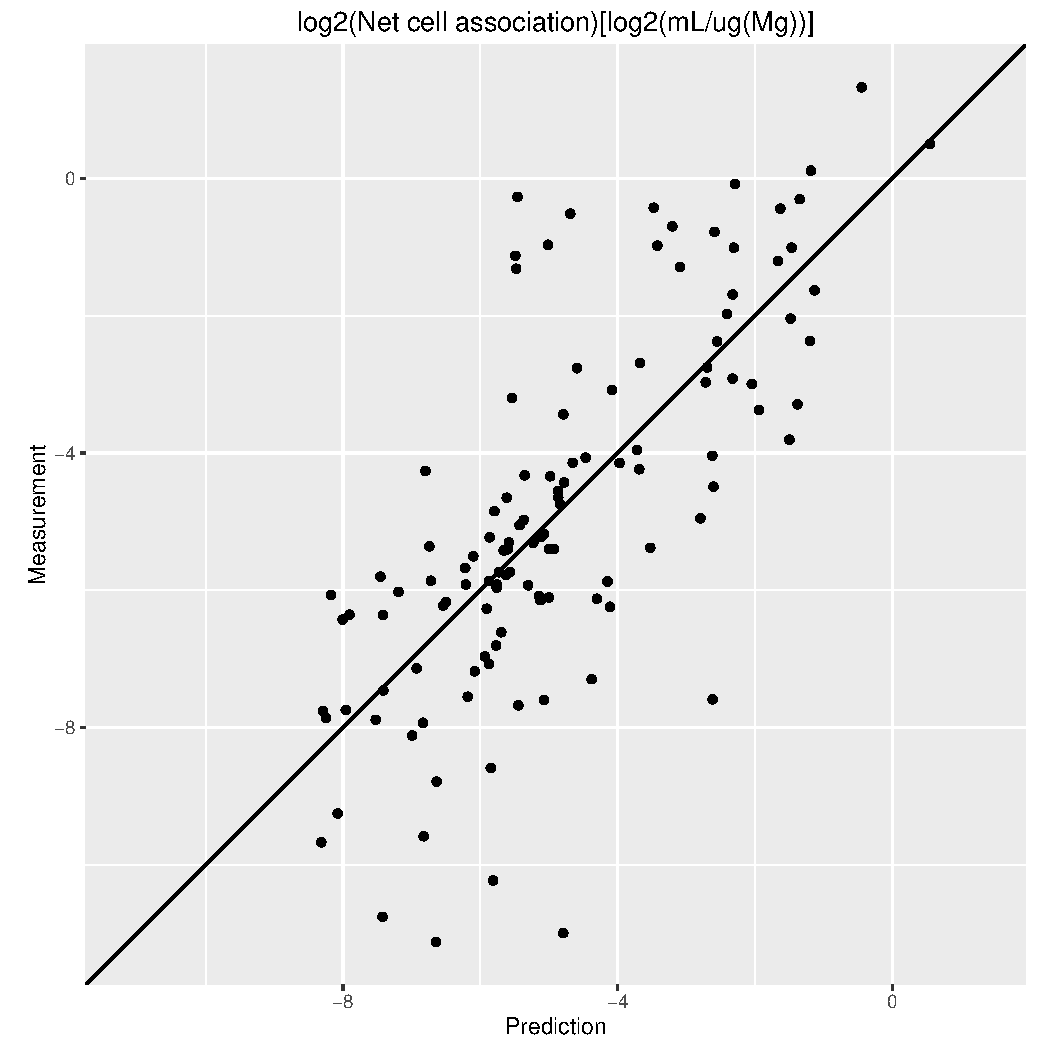
\includegraphics[width=0.3000\textwidth]{figures/PCHEM-rf-0.pdf}\label{fig:pchem0}
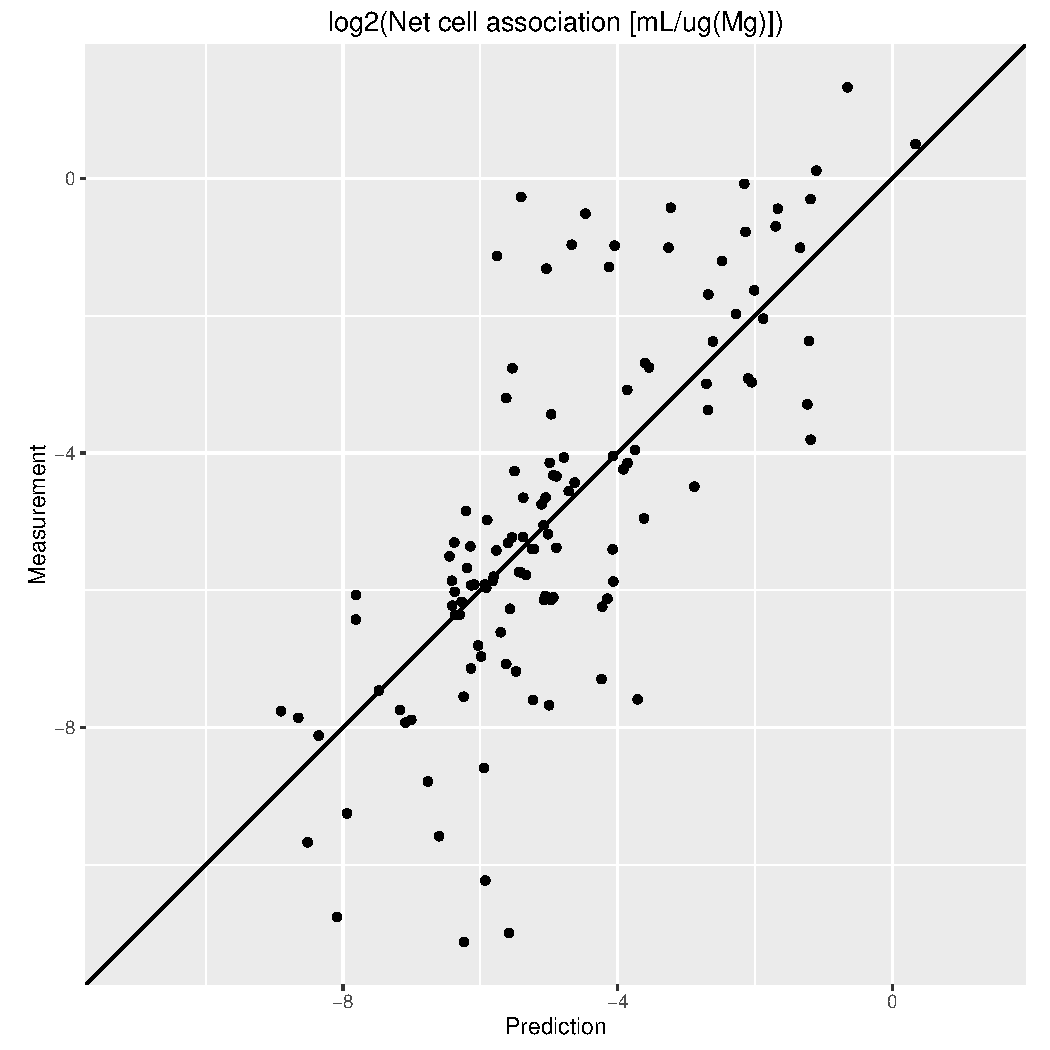
\includegraphics[width=0.3000\textwidth]{figures/PCHEM-rf-1.pdf}\label{fig:pchem1}
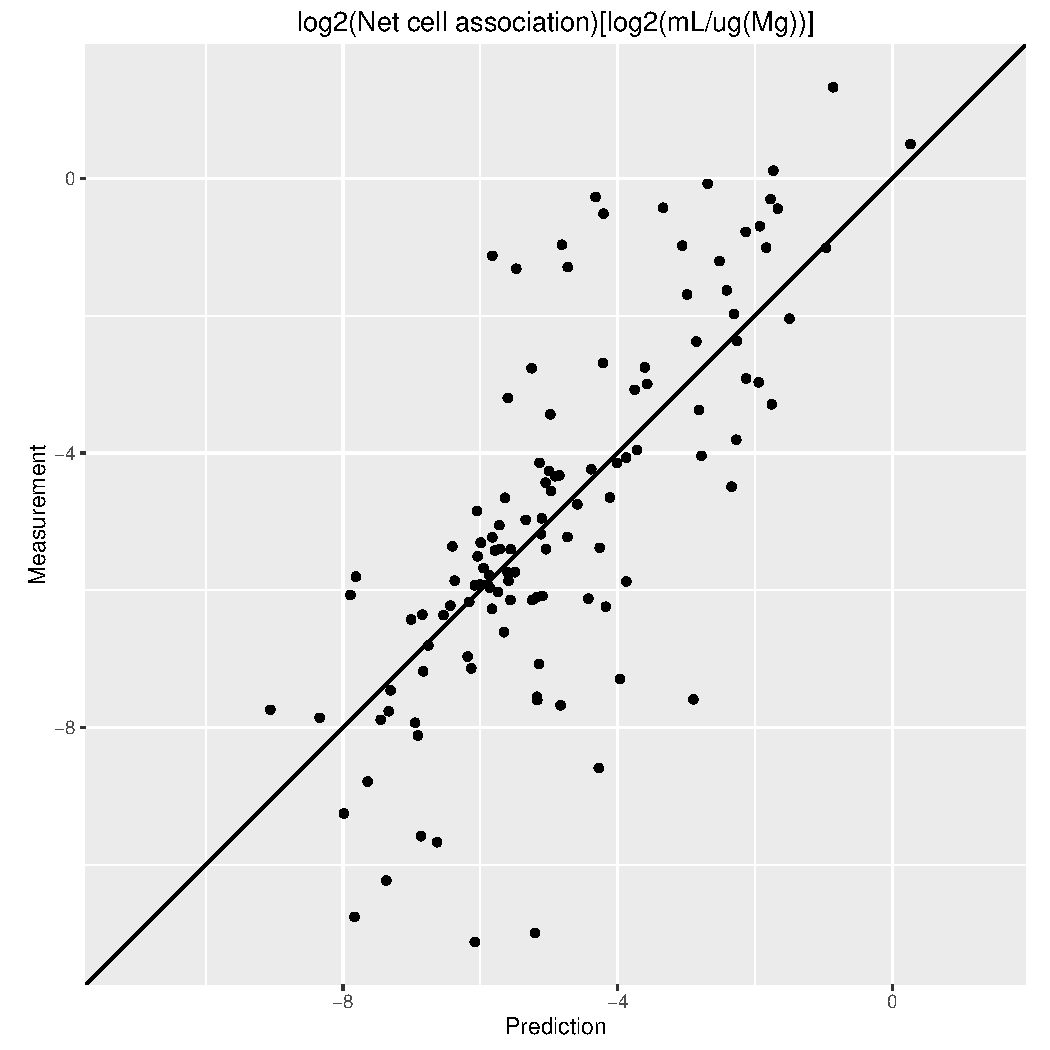
\includegraphics[width=0.3000\textwidth]{figures/PCHEM-rf-2.pdf}\label{fig:pchem2}
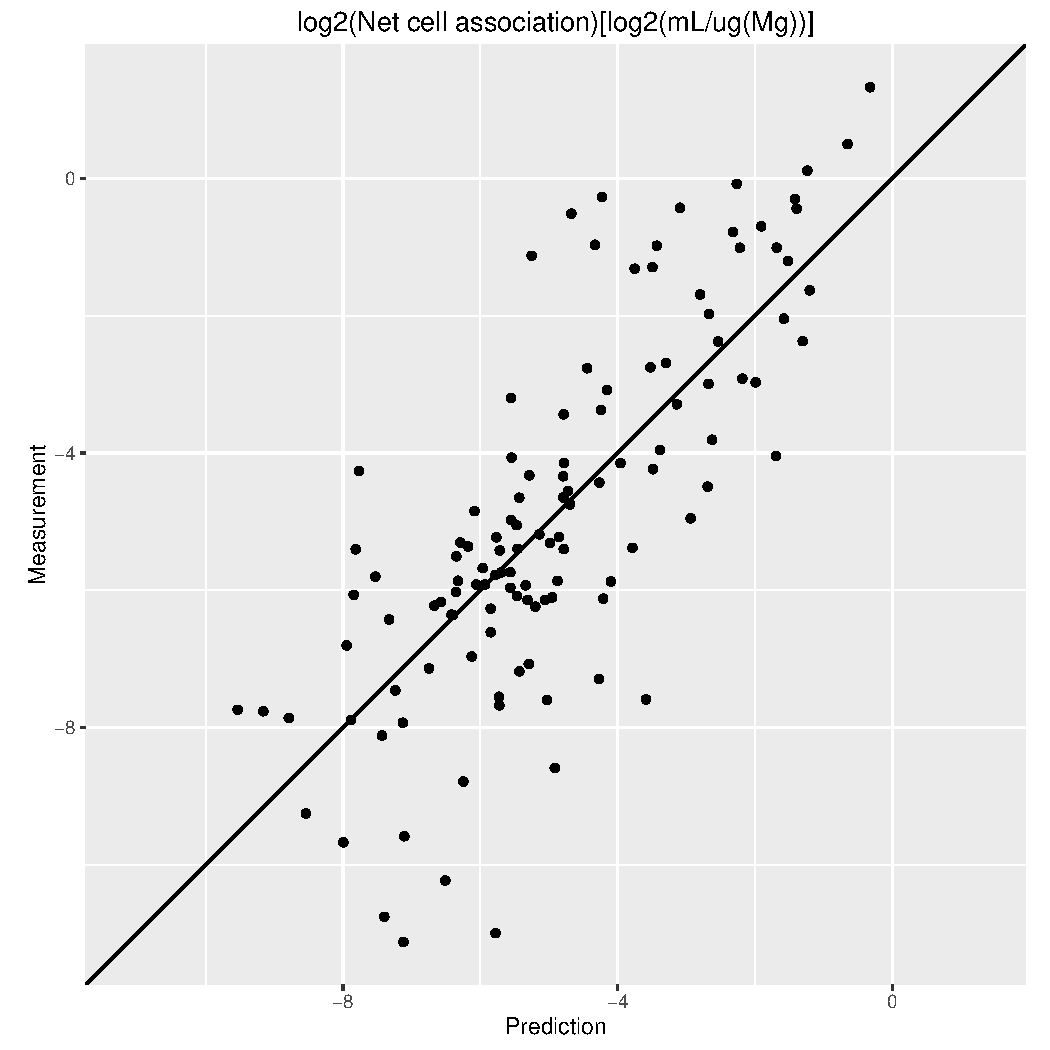
\includegraphics[width=0.3000\textwidth]{figures/PCHEM-rf-3.pdf}\label{fig:pchem3}
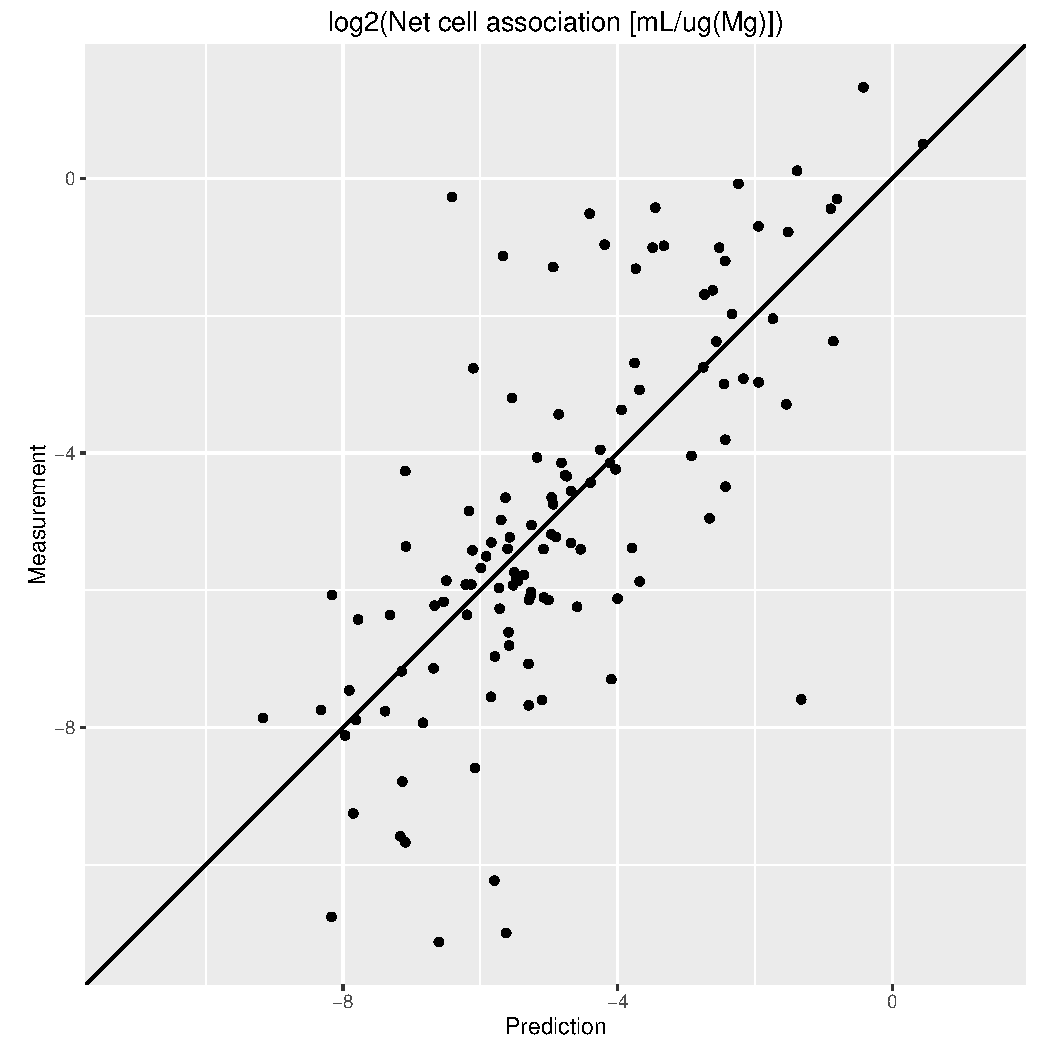
\includegraphics[width=0.3000\textwidth]{figures/PCHEM-rf-4.pdf}\label{fig:pchem4}

\caption{Correlation of predicted vs.~measured values for five
independent crossvalidations with \emph{P-CHEM} descriptors and local
\emph{random forest} models}

\label{fig:pchem}

\end{figure}

\begin{figure}[H]

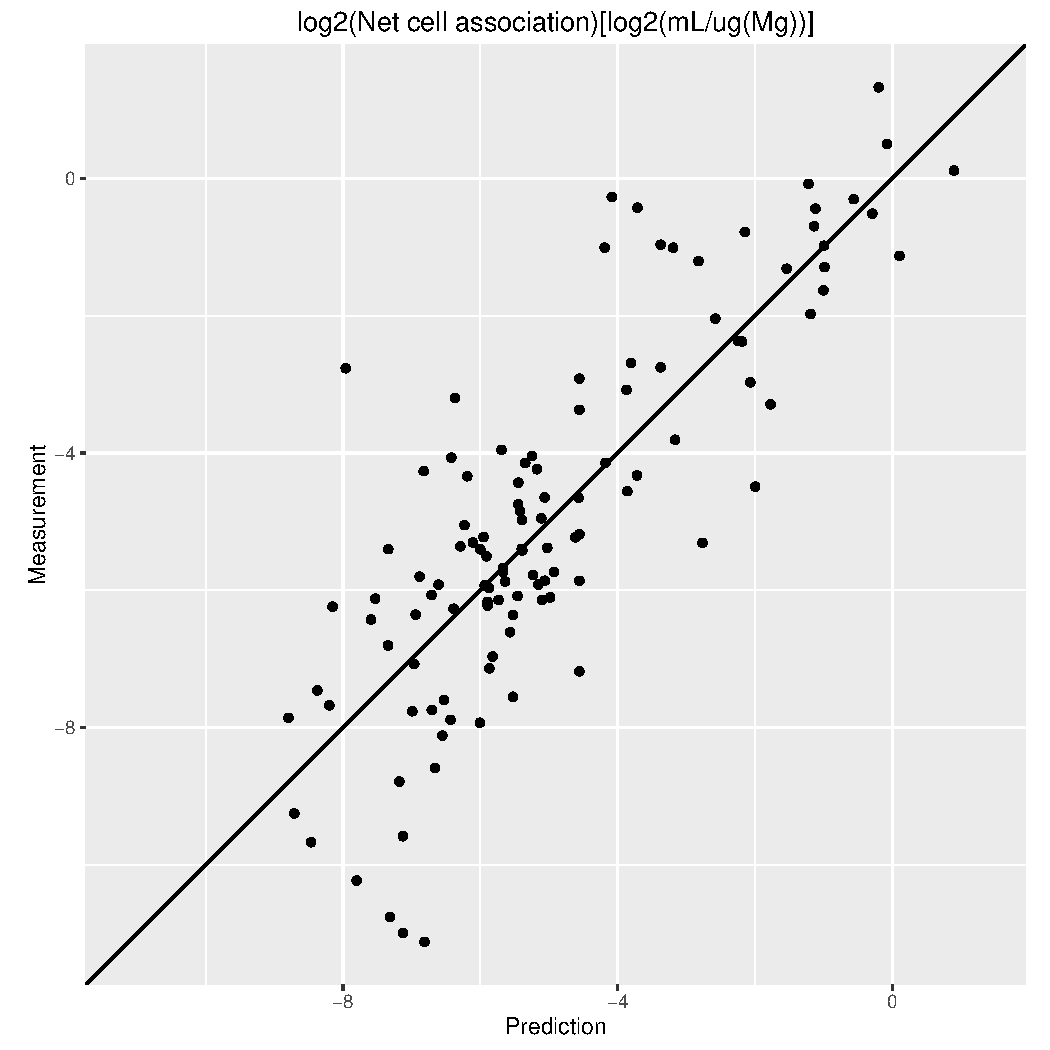
\includegraphics[width=0.3000\textwidth]{figures/Proteomics-rf-0.pdf}\label{fig:prot0}
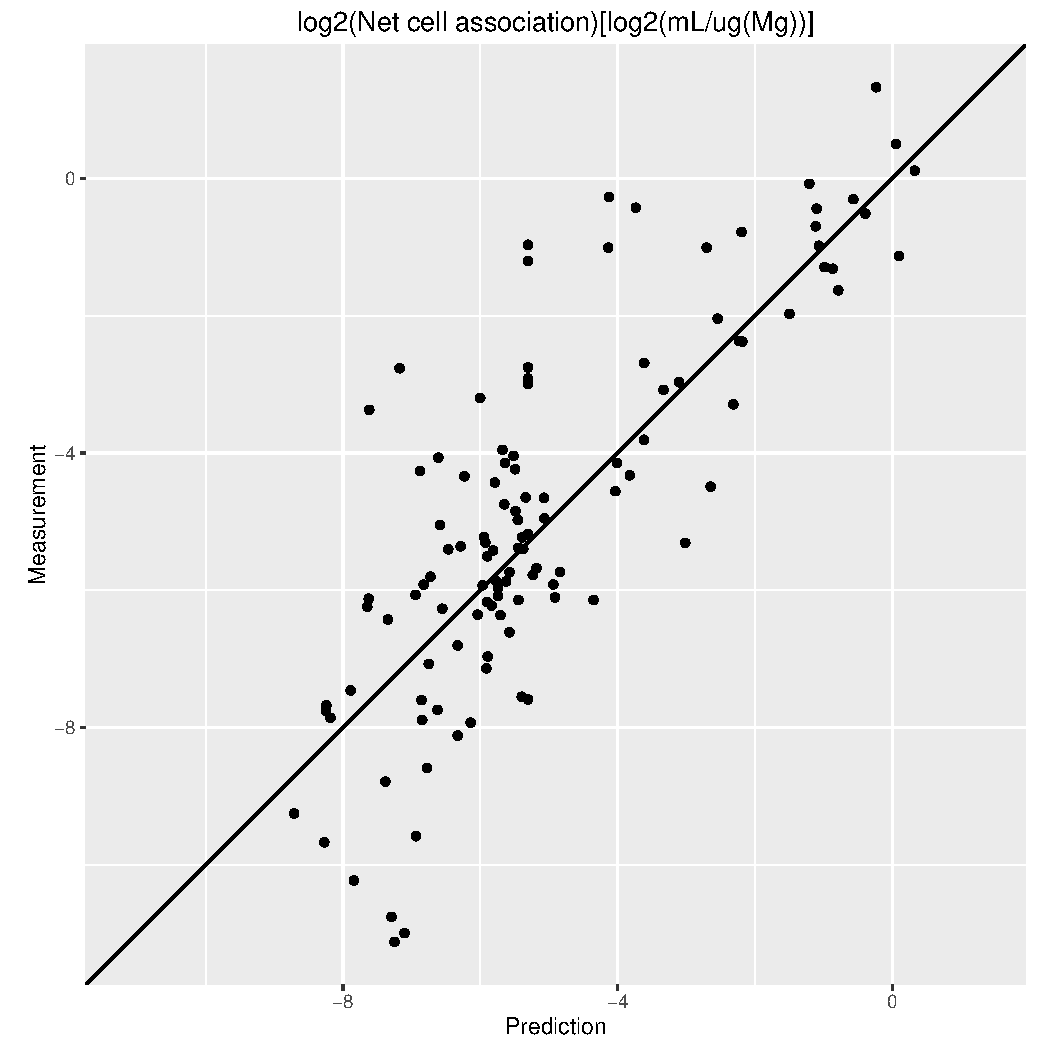
\includegraphics[width=0.3000\textwidth]{figures/Proteomics-rf-1.pdf}\label{fig:prot1}
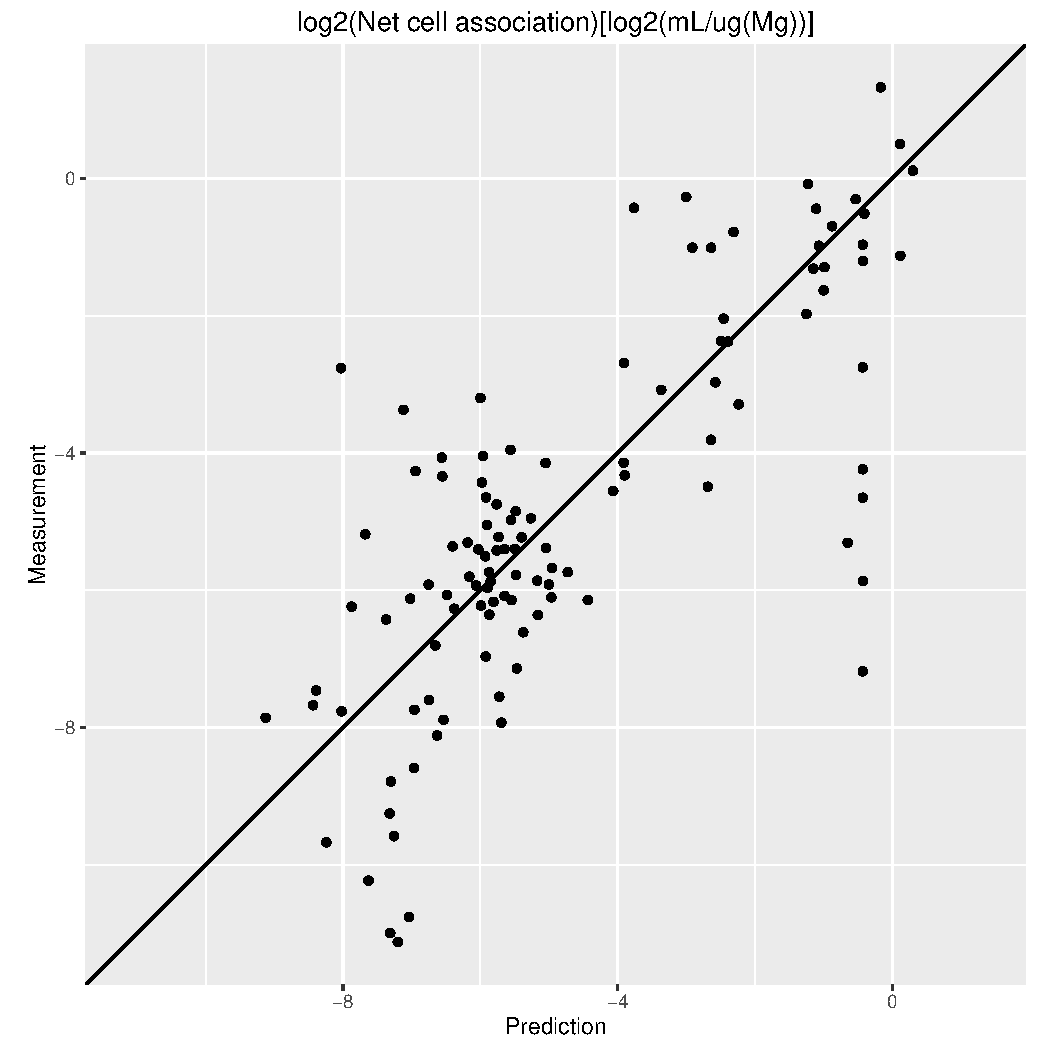
\includegraphics[width=0.3000\textwidth]{figures/Proteomics-rf-2.pdf}\label{fig:prot2}
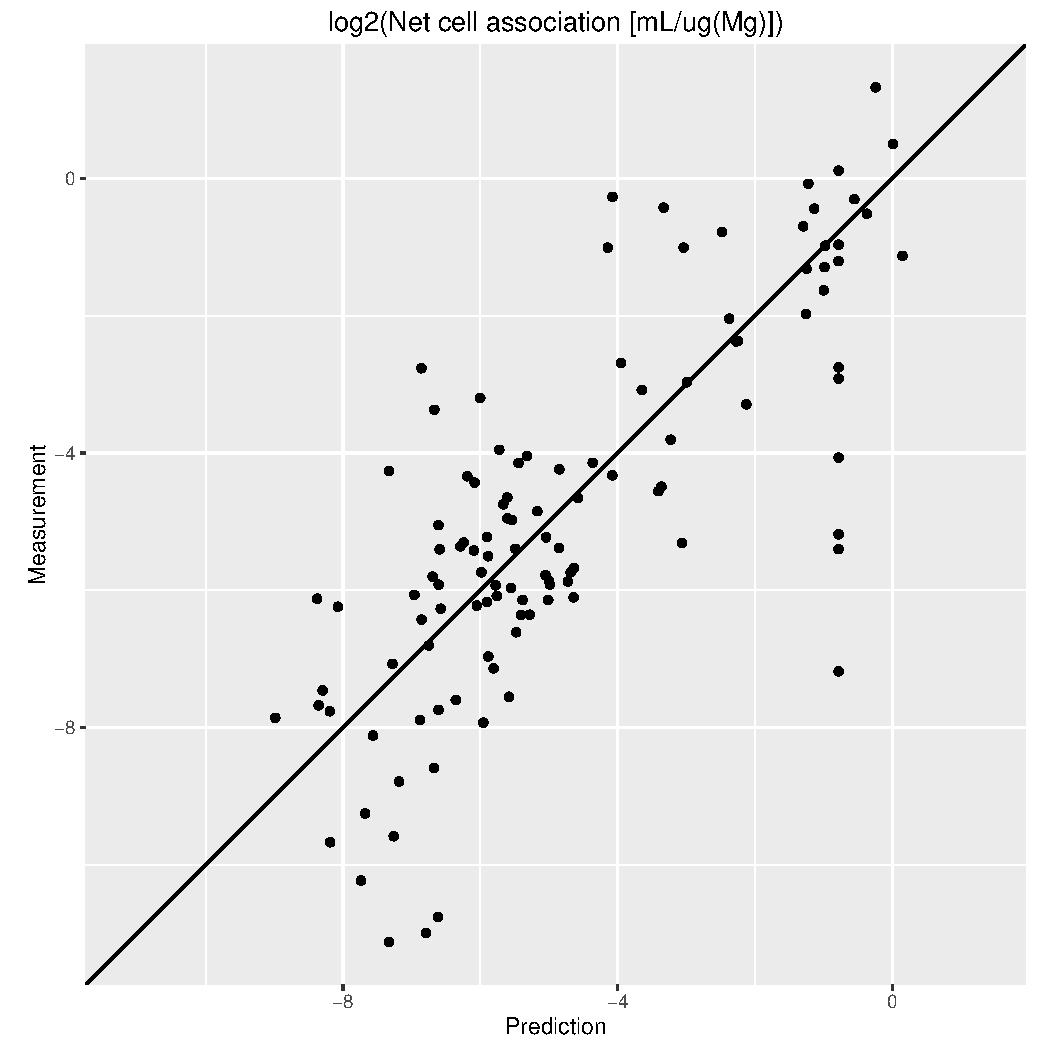
\includegraphics[width=0.3000\textwidth]{figures/Proteomics-rf-3.pdf}\label{fig:prot3}
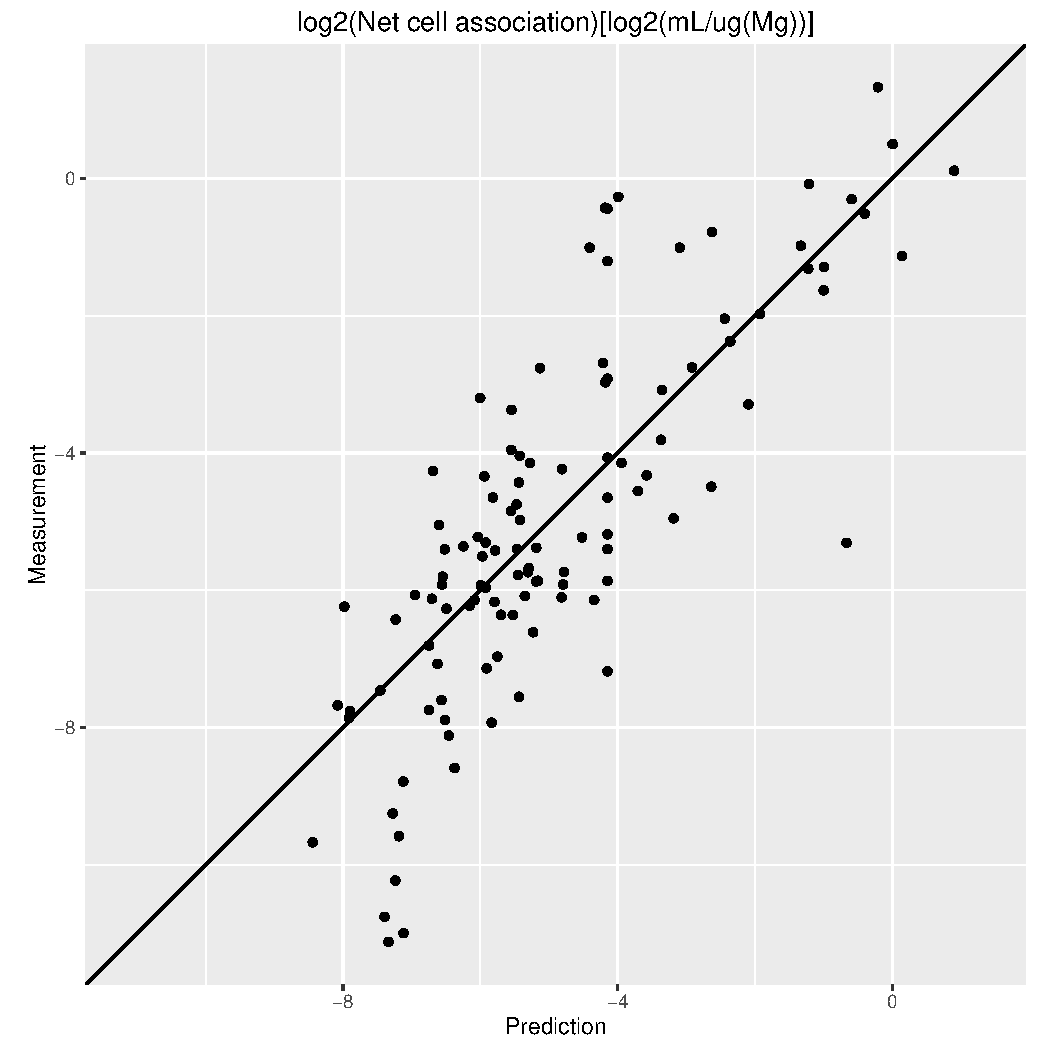
\includegraphics[width=0.3000\textwidth]{figures/Proteomics-rf-4.pdf}\label{fig:prot4}

\caption{Correlation of predicted vs.~measured values for five
independent crossvalidations with \emph{Proteomics} descriptors and
local \emph{random forest} models}

\label{fig:prot}

\end{figure}

\end{document}
